\documentclass[aspectratio=169,11pt,hyperref={colorlinks=true}]{beamer}
\usetheme{boxes}
\setbeamertemplate{navigation symbols}{}
\definecolor{openstack}{RGB}{149,0,4}
\setbeamercolor{titlelike}{fg=openstack}
\setbeamercolor{structure}{fg=openstack}
\hypersetup{colorlinks,urlcolor=openstack}
\setbeamertemplate{footline}[frame number]
% Inserting graphics
\usepackage{graphicx}
% Side-by-side figures, etc
\usepackage{subfigure}
% Code snippits
\usepackage{listings}
% Color stuff
\usepackage{color}
\usepackage{amsmath}
\usepackage{tikz}
\usepackage{tipa}
\newcommand\RBox[1]{%
  \tikz\node[draw,rounded corners,align=center,] {#1};%
}
\usepackage{hyperref}
%\usecolortheme{buzz}
%\usecolortheme{wolverine}
%\usetheme{Boadilla}
\usepackage[T1]{fontenc}

\definecolor{mygreen}{rgb}{0,0.6,0}
\definecolor{mygray}{rgb}{0.5,0.5,0.5}
\definecolor{mymauve}{rgb}{0.58,0,0.82}

\lstset{ %
  backgroundcolor=\color{white},   % choose the background color; you must add \usepackage{color} or \usepackage{xcolor}
  breakatwhitespace=false,         % sets if automatic breaks should only happen at whitespace
  breaklines=true,                 % sets automatic line breaking
  captionpos=b,                    % sets the caption-position to bottom
  commentstyle=\color{openstack},  % comment style
  extendedchars=true,              % lets you use non-ASCII characters; for 8-bits encodings only, does not work with UTF-8
  keepspaces=true,                 % keeps spaces in text, useful for keeping indentation of code (possibly needs columns=flexible)
  keywordstyle=\color{blue},       % keyword style
  otherkeywords={*,...},           % if you want to add more keywords to the set
  numbersep=5pt,                   % how far the line-numbers are from the code
  numberstyle=\tiny\color{mygray}, % the style that is used for the line-numbers
  rulecolor=\color{black},         % if not set, the frame-color may be changed on line-breaks within not-black text (e.g. comments (green here))
  showspaces=false,                % show spaces everywhere adding particular underscores; it overrides 'showstringspaces'
  showstringspaces=false,          % underline spaces within strings only
  showtabs=false,                  % show tabs within strings adding particular underscores
  stringstyle=\color{openstack},   % string literal style
}

\setbeamerfont{caption}{series=\normalfont,size=\fontsize{6}{8}}
\setbeamertemplate{caption}{\raggedright\insertcaption\par}

\setlength{\abovecaptionskip}{0pt}
\setlength{\floatsep}{0pt}

\author[Andrea Frittoli]{%
    \texorpdfstring{
        \begin{columns}
            \column{.45\linewidth}
            \centering
            Andrea Frittoli\\
            \href{mailto:andrea.frittoli@gmail.com}{andrea.frittoli@gmail.com}\\
            \texttt{andreaf on Freenode}\\
            \texttt{@blackchip76 on Twitter}
        \end{columns}
   }
   {Andrea Frittoli}
}
\date{Jun 2, 2017}

\title[Testing at Scale
\hspace{2em}\insertframenumber/\inserttotalframenumber]{Testing at Scale}

\begin{document}

{
\setbeamertemplate{background canvas}{
\includegraphics[width=\paperwidth,height=\paperheight]{background_title.png}}
\setbeamertemplate{footline}{}
\begin{frame}[noframenumbering]
    \setbeamercolor{titlelike}{fg=white}
    \setbeamercolor{structure}{fg=white}
    \setbeamercolor{normal text}{fg=white}
    \hypersetup{colorlinks,urlcolor=white}
    \setbeamercolor{author}{fg=white}
    \setbeamercolor{date}{fg=white}
    \setbeamercolor{background}{bg=openstack}
    \titlepage{}
    \centering
    \href{https://github.com/andreafrittoli/tempest\_at\_scale}{https://github.com/andreafrittoli/testing\_at\_scale}
\end{frame}
}

\begin{frame}
    \frametitle{OpenStack CI in Numbers}
    \begin{figure}
    \begin{center}
    	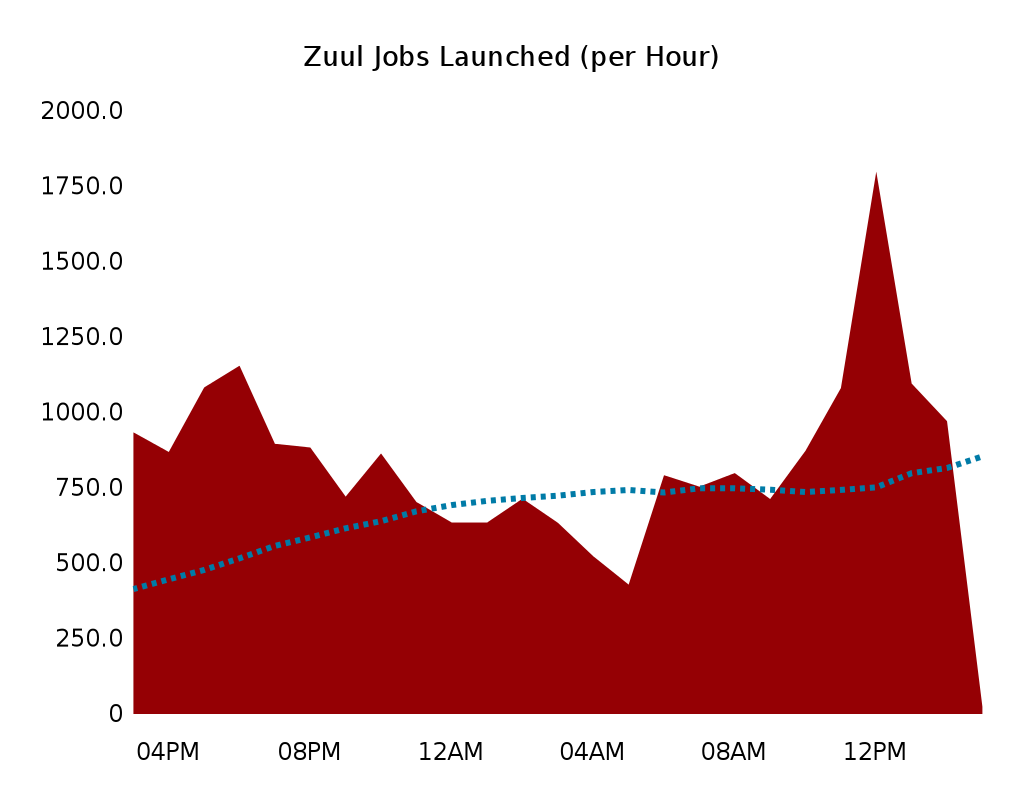
\includegraphics[width=0.5\textwidth]{zuul_all_jobs.png}
         \caption{Source: Zuul, Graphite}
    \end{center}
    \end{figure}
    \begin{itemize}
        \item{2nd graph?}
    \end{itemize}
\end{frame}

\begin{frame}
    \frametitle{Life as a contributor}
    \begin{figure}
    \begin{center}
    	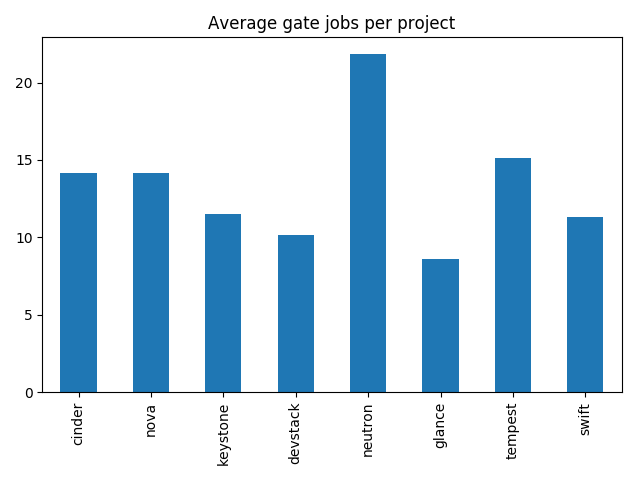
\includegraphics[width=0.5\textwidth]{gate_jobs.png}
         \caption{Source: subunit2sql DB}
    \end{center}
    \end{figure}
    \begin{itemize}
        \item{Graph about number of jobs per patch-set}
        \item{Graph about average number of patch-sets}
    \end{itemize}
\end{frame}

\begin{frame}
    \frametitle{My day in reviews}
    \begin{itemize}
        \item{Pciture about patch size}
        \item{Example of patch that passes the gate but stops running tests}
    \end{itemize}
\end{frame}

\begin{frame}
    \frametitle{Keep the gate flowing}
    \begin{itemize}
        \item{List of gate issues at beginning of pike}
    \end{itemize}
\end{frame}

\begin{frame}
    \frametitle{How it works}
    \begin{itemize}
        \item{TBD}
    \end{itemize}
\end{frame}

\begin{frame}
    \frametitle{Data!}
    \begin{itemize}
        \item{Logs and their size in integration gate}
        \item{Test result data}
        \item{Zuul data}
    \end{itemize}
\end{frame}

\begin{frame}
    \frametitle{Beyond the gate}
    \begin{itemize}
        \item{Periodic jobs}
    \end{itemize}
\end{frame}

\begin{frame}
    \frametitle{Tools}
    \begin{itemize}
        \item{TBD}
    \end{itemize}
\end{frame}

\begin{frame}
    \frametitle{More Automation}
    \begin{itemize}
        \item{TBD}
    \end{itemize}
\end{frame}

\begin{frame}
    \frametitle{Deeper into data}
    \begin{itemize}
        \item{TBD}
    \end{itemize}
\end{frame}

\begin{frame}
    \frametitle{Playing with AI}
    \begin{itemize}
        \item{TBD}
    \end{itemize}
\end{frame}

\section{Questions}
\begin{frame}[c]
    %\frametitle{Questions?}
    \begin{center}
        \Huge Thank you!\\Questions?
    \end{center}
\end{frame}

\end{document}
